\chapter{Results}
The systems works quite well within most of the requirements from specification although not all specifications have been completely fulfilled. The precision is not within 5 cm but rather 10 cm, but this could have easily been calibrated. The system updated around 12 times a second which is somewhat real time. This could have also been improved but wasn't really necessary.\\
The final result is shown on figure~\ref{fig:totalsys}. A graphical presentation of our results is shown in table~\ref{table:alltest}
\begin{figure}[hbpt]
\centering
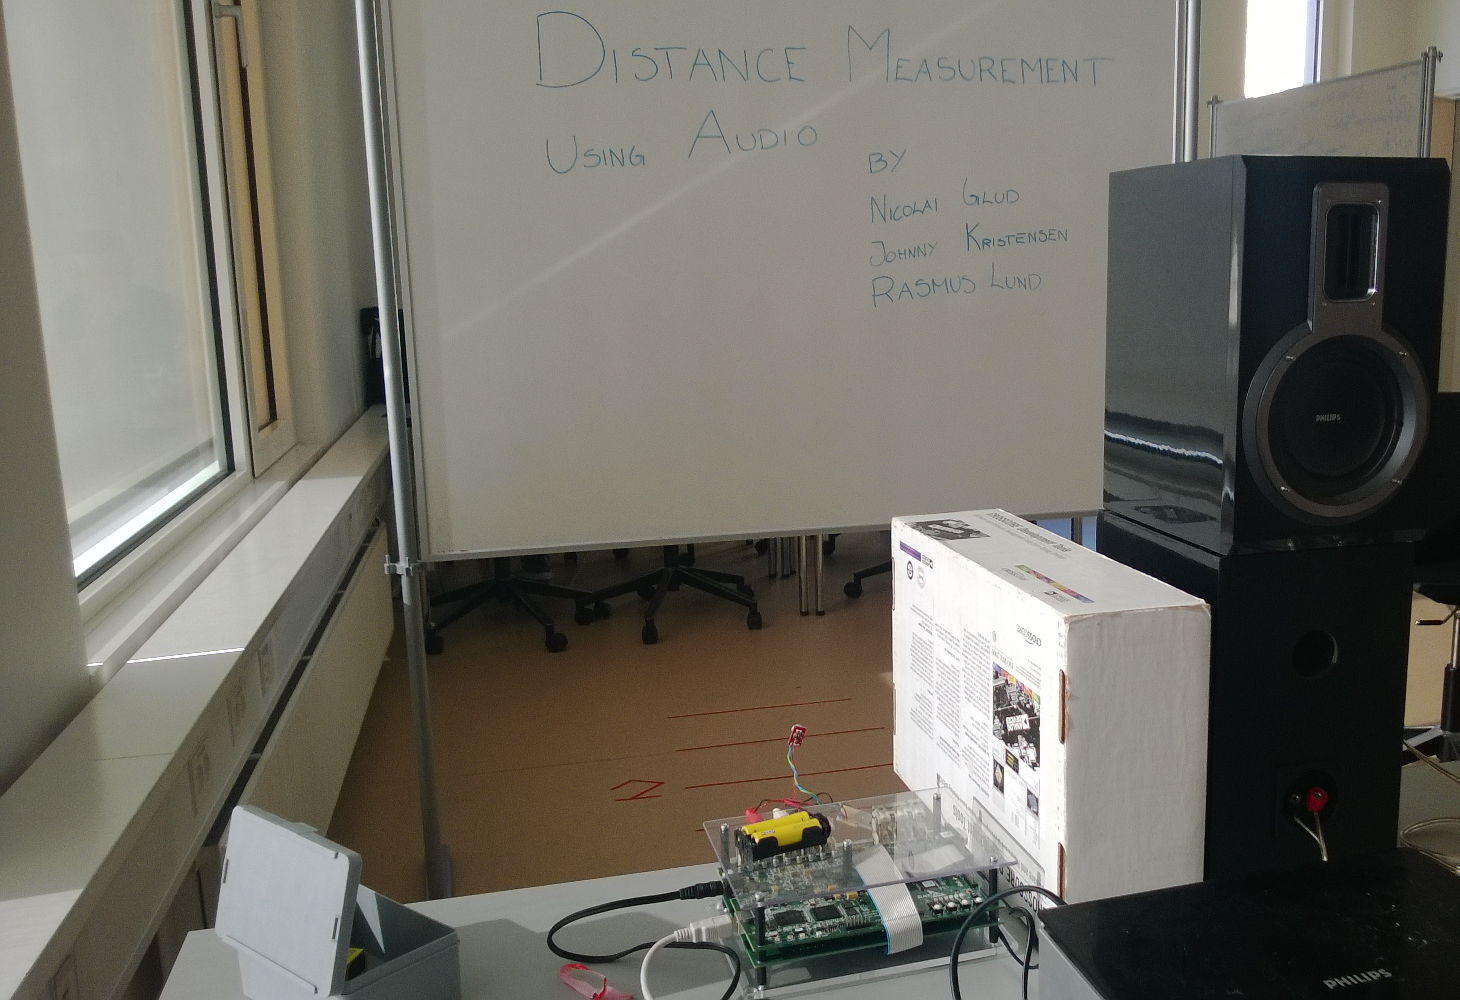
\includegraphics[scale=0.2]{billeder/totalsys}
\caption{Total system}
\label{fig:totalsys}
\end{figure}

\begin{table}[H]
\centering
\begin{tabular}{c c c c}
\hline
Approved & Approved with comment & Not approved & Not tested \\
$\surd$ & $\times$ & $\div$ & $\diamond$ \\\hline
\end{tabular}
\caption{Test Approval Categories}
\end{table}

\begin{table}[H]
\centering
\begin{tabular}{ c c c }
\hline
Requirement: & Status & Comment \\ \hline
Use of DSP & $\surd$ \\
Sound output & $\surd$ \\
Sound input & $\surd$ \\
Precision: <5 cm & $\times$ & <10 cm which is acceptable for now \\
Range: 25cm - 250 cm & $\surd$ \\
Frequency band: 14 - 16 kHz & $\surd$ \\
Memory: max 32kB & $\surd$ \\
System must be real-time & $\times$ & Acceptable for now \\ \hline
\end{tabular}
\caption{Requirement results}
\label{table:alltest}
\end{table}

\chapter{Improvements}
This chapter contains thoughs about the improvements we want to make to our system but did not have the time to do.
\section{Using the system as an actual musical instrument}
\subsection{Playing notes}
The system outputs a sine wave sound. This is great for demonstrative purposes but might not be as pleasant to listen to. What makes a musical sound or "note" pleasant to listen to is harmonics. Most musical tones are composed of fundamental tone and multiple overtones. A sequence of a fundamental tone and 3 overtones would then consist of 4 harmonics. Mathematically, tones are composed of the fundamental frequency and multiples of fundamental frequency like so:\\
\begin{itemize}
\item 1 * freq : fundamental tone : 1st harmonic
\item 2 * freq : 1st overtone     : 2nd harmonic
\item 3 * freq : 2nd overtone     : 3rd harmonic
\item n * freq : (n-1) overtone   : nth harmonic
\end{itemize}
This is also shows on figure ~\ref{fig:harmonics}. To produce such a signal on an embedded unit we would have to use the principle of Fourier series and add the different frequency components together. 
\begin{figure}[hbpt]
\centering
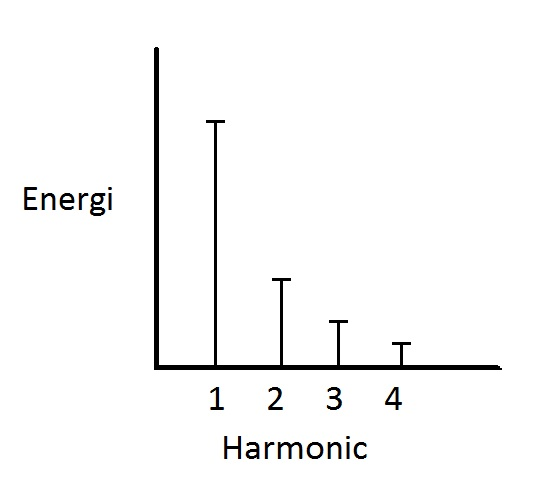
\includegraphics[scale=0.5]{billeder/harmonics}
\caption{n = 4 : harmonics}
\label{fig:harmonics}
\end{figure}
\subsection{Select distance intervals equal to notes}
The idea would be to set intervals for distance much like the distance between keys on a piano. This is shown on figure~\ref{fig:pianokeys}. The idea would then be that you would place a person or an item in the interval and then play a tone with a fixed rate. The rates would then be configurable with buttons on the blackfin for instance.
\begin{figure}[hbpt]
\centering
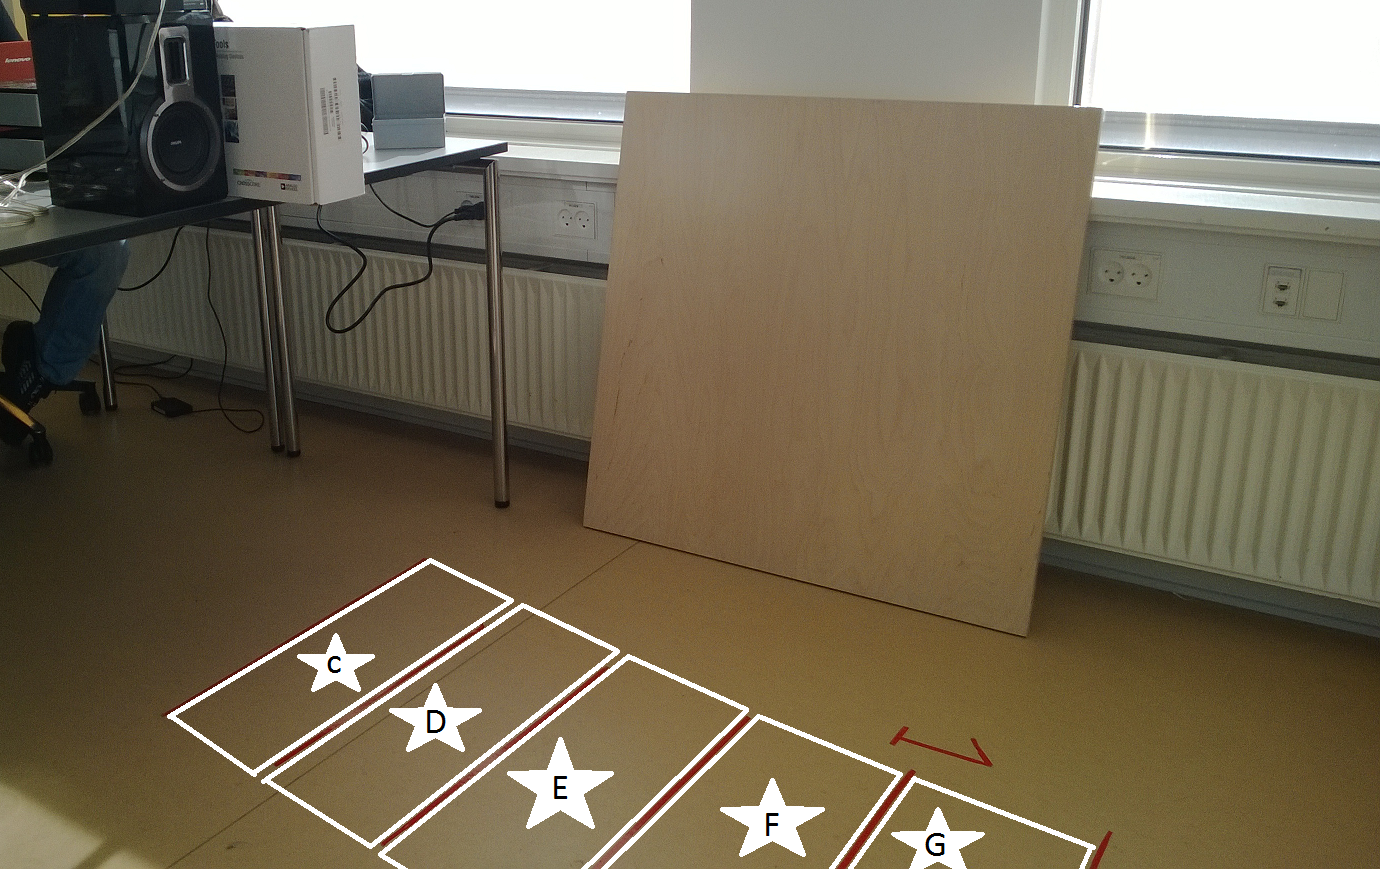
\includegraphics[scale=0.3]{billeder/pianokeyground}
\caption{Piano Keys drawn in front of the system}
\label{fig:pianokeys}
\end{figure}
\section{Buffers sizes}
In this project we went along with somewhat "random" sizes of buffers for our signals. We used a good rule of thumb and chose some sizes we know would be sufficient. 
This comes as a disadvantage which we chose not to develop a solution for and that is the computation time.
 By only using buffers which can hold samples representing the maximum time the sound would travel, we could use the time of which we record and the time it would take to compute the correlation of the signals.\\
An optimal size of buffer for a max distance of 250 cm would be:\\
\begin{equation}
\frac{\frac{buffer\ size}{48000Hz}*343\frac{m}{s}}{2}=250cm
\end{equation}
Solve for buffer size and we get ~700 samples. So 700 samples at 48000Hz would give the sound time to travel 2*250cm which would be the minimum size of our buffer if we have to meet the demand of a maximum distance measurement of 250cm from the specification.
\section{Doppler effect}
During our various tests we found that our system was sensitive to the vibration of the wooden plate on which we bounced our signal. Below is a plot of our distance measurements over 30 measurements.\\
\begin{figure}[H]
\centering
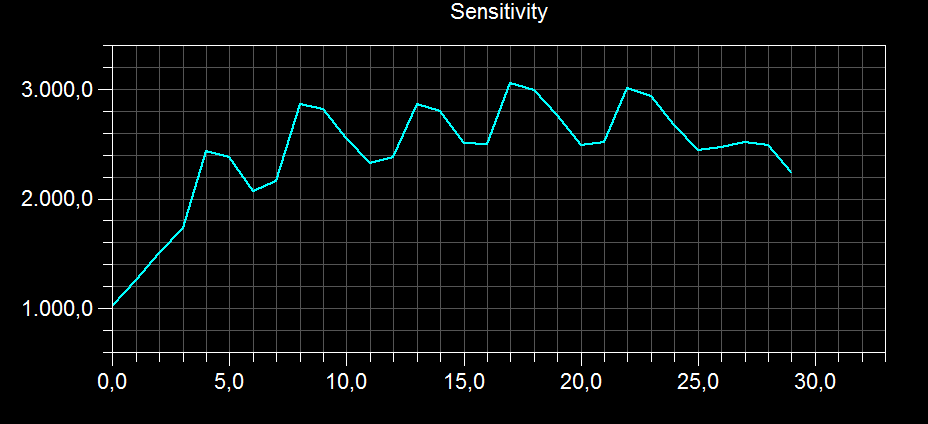
\includegraphics[width=.8\textwidth]{billeder/sensitivity}
\caption{sensitivity plot from VisualDSP++}
\end{figure}
We think the doppler effect is a big part of the issue here. According to wikipedia\footnote{\url{http://en.wikipedia.org/wiki/Doppler_effect}} the change in frequency caused by a velocity on a certain frequency can be easily calculated. Assuming the wood plate travels at 10cm/s (which is pretty slow) the doppler effect would change the frequency with around 4.5Hz.\\
To our system this would in fact be interpreted as if the signal arrived earlier then it actually does because the correlation will change. According to some rought calculations this could actually account for more then 50-70cm in displacement of our measurements.\\
This is not something we can do much to and it surprised the group quite a big deal, we are not entirely convinced this is the entirety of the problem but it is highly likely that it has a noticeable impact.\\
\section{speaker/microphone angle}
Another optimization/improvement problem is caused by the angel on which the signal hits the wooden plate because the microphone and speaker cannot be placed within each other. Below on the left is a sketch of how the signal hits at an angel and how the calculated distance and the actual distance is different. On the right is a graph showing the calculated distance compared to the actual distance.
\begin{figure}[H]
\begin{minipage}[b]{0.49\linewidth}
\centering
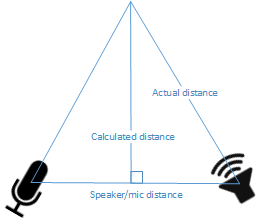
\includegraphics[width=1\textwidth]{billeder/angle_error}
\caption{Angle figure}
\end{minipage}
\hspace{0.5cm}
\begin{minipage}[b]{0.49\linewidth}
\centering
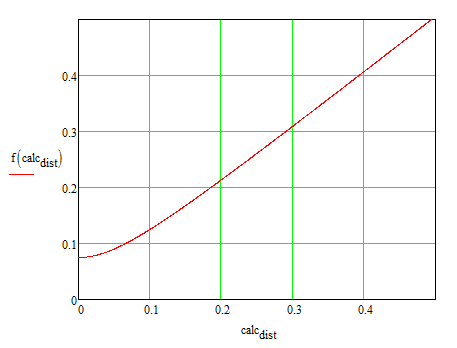
\includegraphics[width=1\textwidth]{billeder/angle_graph}
\caption{Angle graph}
\end{minipage}
\end{figure}
As shown in the graph the impact is only significant at very short distances (0-25cm). Therefore we do not take this effect into account.\\
The function for the graph is(by the principle of our dear friend Pythagoras):\begin{equation}
\sqrt{\left(\frac{speaker/mic\ distance}{2}\right)^2+calculated\ distance^2}=acutal\ distance
\end{equation}